\documentclass[tikz,border=8pt]{standalone}
\usepackage{amsmath,amssymb}
\usetikzlibrary{arrows.meta,automata,positioning,quotes}
\begin{document}
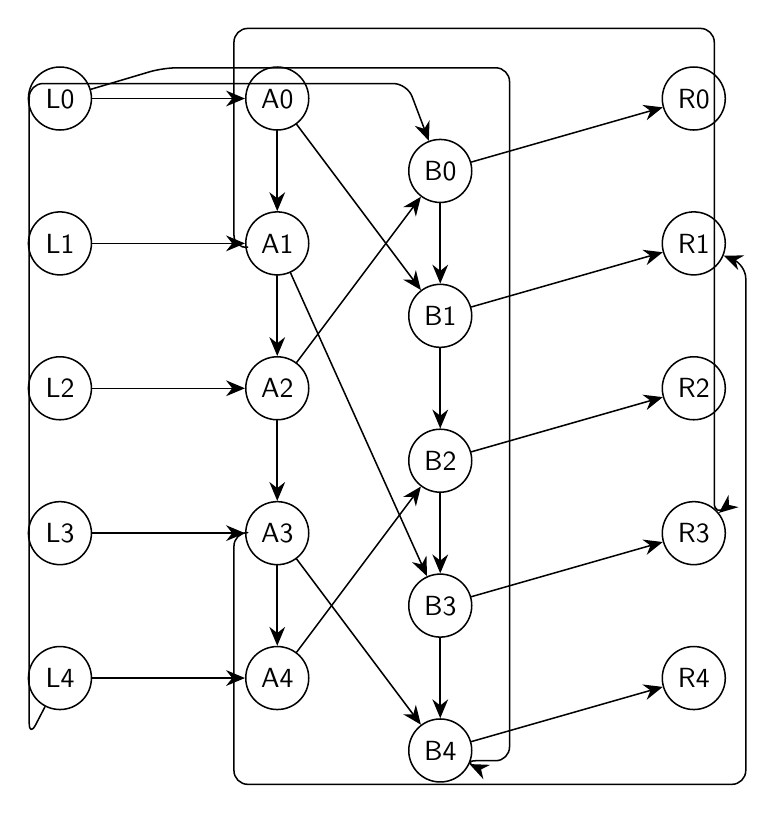
\begin{tikzpicture}[x=1cm,y=1cm]
\tikzset{
  graphnode/.style={circle,draw=black,line width=0.55pt,minimum size=8mm,inner sep=1pt,font=\sffamily},
  graphedge/.style={draw=black,line width=0.55pt,line cap=round,line join=round},
  directed/.style={graphedge,-{Stealth[length=2.4mm,width=2.0mm]}},
  undirected/.style={graphedge}
}
\node[graphnode] (n_L0) at (-0.51,6.91) {L0};
\node[graphnode] (n_L1) at (-0.51,5.07) {L1};
\node[graphnode] (n_L2) at (-0.51,3.23) {L2};
\node[graphnode] (n_L3) at (-0.51,1.39) {L3};
\node[graphnode] (n_L4) at (-0.51,-0.45) {L4};
\node[graphnode] (n_R0) at (7.54,6.91) {R0};
\node[graphnode] (n_R1) at (7.54,5.07) {R1};
\node[graphnode] (n_R2) at (7.54,3.23) {R2};
\node[graphnode] (n_R3) at (7.54,1.39) {R3};
\node[graphnode] (n_R4) at (7.54,-0.45) {R4};
\node[graphnode] (n_A0) at (2.25,6.91) {A0};
\node[graphnode] (n_A1) at (2.25,5.07) {A1};
\node[graphnode] (n_A2) at (2.25,3.23) {A2};
\node[graphnode] (n_A3) at (2.25,1.39) {A3};
\node[graphnode] (n_A4) at (2.25,-0.45) {A4};
\node[graphnode] (n_B0) at (4.32,5.99) {B0};
\node[graphnode] (n_B1) at (4.32,4.15) {B1};
\node[graphnode] (n_B2) at (4.32,2.31) {B2};
\node[graphnode] (n_B3) at (4.32,0.47) {B3};
\node[graphnode] (n_B4) at (4.32,-1.37) {B4};
\draw[directed] (n_L0) -- (n_A0);
\draw[directed] (n_L1) -- (n_A1);
\draw[directed] (n_L2) -- (n_A2);
\draw[directed] (n_L3) -- (n_A3);
\draw[directed] (n_L4) -- (n_A4);
\draw[directed] (n_B0) -- (n_R0);
\draw[directed] (n_B1) -- (n_R1);
\draw[directed] (n_B2) -- (n_R2);
\draw[directed] (n_B3) -- (n_R3);
\draw[directed] (n_B4) -- (n_R4);
\draw[directed] (n_A0) -- (n_B1);
\draw[directed] (n_A1) -- (n_B3);
\draw[directed] (n_A2) -- (n_B0);
\draw[directed] (n_A3) -- (n_B4);
\draw[directed] (n_A4) -- (n_B2);
\draw[directed] (n_A0) -- (n_A1);
\draw[directed] (n_A1) -- (n_A2);
\draw[directed] (n_A2) -- (n_A3);
\draw[directed] (n_A3) -- (n_A4);
\draw[directed] (n_B0) -- (n_B1);
\draw[directed] (n_B1) -- (n_B2);
\draw[directed] (n_B2) -- (n_B3);
\draw[directed] (n_B3) -- (n_B4);
\draw[directed,rounded corners=5pt] (n_L0) -- (0.80,7.30) -- (5.20,7.30) -- (5.20,-1.50) -- (4.60,-1.50) -- (n_B4);
\draw[directed,rounded corners=5pt] (n_L4) -- (-0.90,-1.20) -- (-0.90,7.10) -- (3.90,7.10) -- (n_B0);
\draw[directed,rounded corners=5pt] (n_A1) -- (1.70,5.00) -- (1.70,7.80) -- (7.80,7.80) -- (7.80,1.60) -- (n_R3);
\draw[directed,rounded corners=5pt] (n_A3) -- (1.70,1.40) -- (1.70,-1.80) -- (8.20,-1.80) -- (8.20,4.80) -- (n_R1);
\end{tikzpicture}
\end{document}
